%
% cwt.tex
%
% (c) 2019 Prof Dr Andreas Müller, Hochschule Rapperswil
%
\section{Stetige Wavelet-Transformation
\label{sextion:cwt}}
\rhead{Stetige Wavelet-Transformation}
Ein Wavelet soll nun dazu verwendet werden, ein Signal $f(t)$ abzutasten.
Da das Wavelet lokalisiert ist, müssen wir es der $t$-Achse entlang
verschieben, um jeden Abschnitt des Signals sinnvoll abtasten zu
können.
Da das Wavelet auch im Frequenzbereich lokalisiert ist, müssen wir
es ausserdem skalieren, um sowohl kurzwellige wie auch langwellige
Details des Signals zu erfassen.

Sei also $\psi$ ein Wavelet und somit eine Funktion, die die
Zulässigkeitsbedingung~\eqref{cwt:zulaessig} erfüllt\footnote{Die nachfolgenden
Definitionen sind zum Teil auch sinnvoll, wenn die Zulässigkeitsbedingung
nicht erfüllt ist, doch ist die so entstehende Transformation nicht unbedingt
stetig oder umkehrbar.}.
Wir setzen daher
\[
\psi_{a,b}(t)
=
\frac{1}{\sqrt{|a|}} \psi\biggl(\frac{t-b}a\biggr)
=
T_bD_a\psi (t).
\]
Den Spezialfall $b=0$ kürzen wir $\psi_a = \psi_{a,0}$ ab.

\begin{lemma}
Die verschobenen und gestreckten Kopien $\psi_{a,b}$ von $\psi$ haben alle
die gleiche Norm: $\|\psi_{a,b}\|=1$.
\end{lemma}

\begin{proof}[Beweis]
Dies folgt unmittelbar aus der in Kapitel~\ref{chapter:fourier}
hergeleiteten Tatsache, dass die Operatoren $T_b$ und $D_a$
Isometrien von $L^2(\mathbb R)$ sind.
\end{proof}

\begin{beispiel}
Bei den Haar-Wavelets haben wir als Streckungsfaktoren die Zweierpotenzen
$2^j$ mit $j\in\mathbb Z$ verwendet.
Damit alle Wavelets die gleiche Norm bekamen, haben wir mit dem Faktor
$2^{-j/2}$ kompensiert.
Ausgehend vom Haar-Mutterwavelet
\[
\psi_{\text{Haar}} = \chi_{[0,\frac12)} - \chi_{[\frac12,1)}
\]
ist das skalierte und verschobene Wavelet
$\psi_{\text{Haar},a,b}$ eine stückweise konstante Funktion,
die für $a>0$ beim Punkt $b$ auf den Wert $1/\sqrt{|a|}$ springt,
beim Punkt $b+a/2$ auf $-1/\sqrt{|a|}$ und ab $b+a$ wieder verschwindet.
Der Träger der Funktion $\psi_{\text{Haar},a,b}$ ist also das Intervall
$[b,b+a]$.
% XXX Abbildung für das skalierte  Haar-Wavelet
\end{beispiel}

%\begin{beispiel}
%Sei $\psi=\frac1{\sqrt{2\pi}} e^{-t^2/2}$ die Wahrscheinlichkeitsdichte
%der Standardnormalverteilung.
%Man kann nachrechnen, dass $\psi$ die Zulässigkeitsbedingung erfüllt. 
%%TODO: \int \psi = 1 \ne 0! Normalverteilungen sind keine Wavelets
%Die $\sigma$ skalierten und um $\mu$ verschobenen Funktionen sind
%\[
%\psi_{\sigma,\mu}(t)
%=
%\frac{1}{\sqrt{2\pi\sigma}} e^{-(t-b)^2/2\sigma^2},
%\]
%die Wahrscheinlichkeitsdichte einer Normalverteilung mit Erwartungswert $\mu$
%und Varianz $\sigma^2$.
%\end{beispiel}

Die skalierten und verschobenen Funktionen $\psi_{a,b}$ können jetzt als
Analyse-Funktionen für das Signal dienen.

\begin{definition}
\label{cwt:definition}
Die {\em stetige Wavelet-Transformation} des Signals $f(t)$ mit dem Wavelet
\index{Wavelet-Transformation, stetige}%
\index{stetige Wavelet-Transformation}%
$\psi$ ist die Funktion
\begin{equation}
\mathcal{W}f (a,b)
=
\langle f,\psi_{a,b}\rangle
=
\frac{1}{\sqrt{|a|}}\int_{-\infty}^\infty f(t)\,\overline{
\psi\biggl(\frac{t-b}{a}\biggr)}\,dt.
\label{cwt:definition:eq}
\end{equation}
Falls in einem Kontext verschiedene Wavelet-Funktionen vorkommen, kann die
Notation eindeutig gemacht werden, indem die Wavelet-Transformation
$\mathcal{W}_{\psi}f$ geschrieben wird.
Der Definitionsbereich der stetigen Wavelet-Transformation ist die Menge
\[
H
=
\mathbb R^2_-
=
\mathbb R^*\times \mathbb R
=
\mathbb R^2 - (\{0\}\times \mathbb R)
\]
die Ebene ohne die Achse $a=0$.
\end{definition}

Die Wavelet-Transformation liefert also eine Funktion von {\em zwei}
Variablen.
Die beiden Parameter erlauben, unabhängig voneinander eine bestimmte
Stelle des Signals genauer anzuschauen durch Wahl von $b$ sowie die
Details genauer aufzulösen durch Vergrösserung von $a$.

Da die stetige Wavelet-Transformation einer Funktion $f$ ein Skalarprodukt
mit einer skalierten und verschobenen Waveletfunktion ist, kann die Skalierung
und Verschiebung auch auf die Funktion $f$ geschoben werden.
Nach Satz~\ref{fourier:satz:adjungierte} gilt
\begin{equation}
\mathcal{W}f(a,b)
=
\langle f,T_bD_a\psi\rangle
=
\langle T_{-b}f,D_a\psi\rangle
=
\langle D_{1/a}T_{-b}f,\psi\rangle
=
\mathcal{W}(D_{1/a}T_{-b})(1,0).
\label{cwt:formel:shift}
\end{equation}
Wir verwenden diese Idee im folgenden Beispiel.

\begin{beispiel}
\begin{figure}
\centering
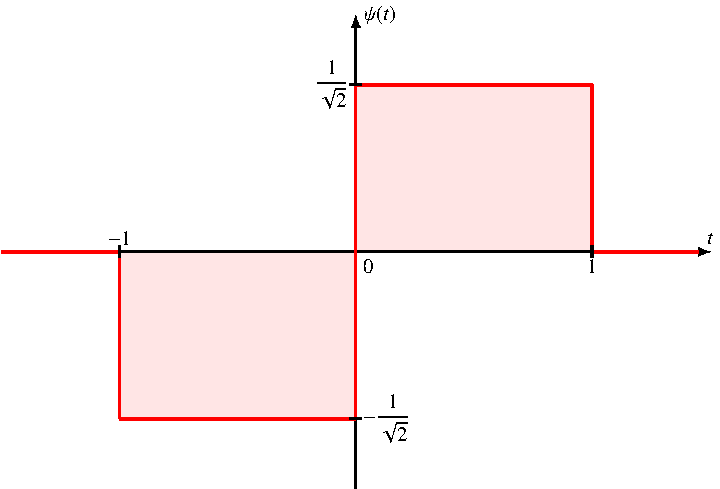
\includegraphics{chapters/4-cwt/images/psigraph.pdf}
\caption{Graph der Funktion $\psi(t)$ für das Beispiel der
Wavelet-Transformation in Abbildung~\ref{cwt:psi-cwt}.
\label{cwt:psi-graph}}
\end{figure}
\begin{figure}
\centering
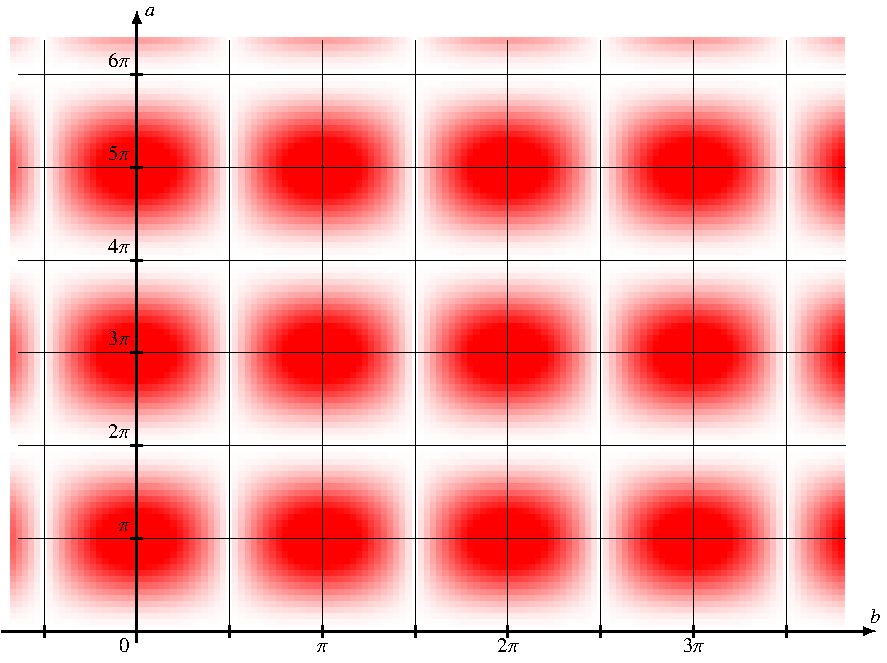
\includegraphics[width=\hsize]{chapters/4-cwt/images/psisin.pdf}
\caption{Wavelet-Transformation der Funktion $f(t)=\sin t$ berechnet
mit dem Wavelet $\psi(t)$ von Abbildung~\ref{cwt:psi-graph}.
Rot steht für positive Werte der Wavelet-Transformation, blau für negative.
\label{cwt:psi-cwt}}
\end{figure}
Der Graph der Funktion ist auch in Abbildung~\ref{cwt:psi-graph} dargestellt.
Wir betrachten die Funktion
\begin{equation}
\psi(t) = \begin{cases}
-\frac1{\sqrt{2}}&\qquad -1\le t< 0\\
\frac1{\sqrt{2}}&\qquad 0\le t< 1\\
0&\qquad\text{sonst}
\end{cases}
\label{cwt:beispiel:psi}
\end{equation}
Dies ist eine gestreckte und verschobene Version des Haar-Wavelets,
und erfüllt daher automatisch die Zulässigkeitsbedingung für ein Wavelet.
Ausserdem gilt $\|\psi\|=1$.
Gegenüber dem Haar-Mutter-Wavelet hat diese Funktion den Vorteil, dass 
sie antisymmetrisch ist, so dass auch die stetige Wavelettransformation
einer antisymmetrischen Funktion wieder symmetrisch sein wird.

Wir berechnen jetzt die stetige Wavelet-Transformat des Signals $f(t)=\sin t$.
Nach Definition und
\eqref{cwt:formel:shift}
ist
\begin{align*}
\mathcal{W}f(a,b)
&=
\langle D_{1/a}T_{-b}f,\psi\rangle
=
\int_{-\infty}^\infty f(at+b) \overline{\psi(t)}\,dt.
\end{align*}
Dies soll jetzt für die oben definierte Funktion $\psi(t)$ durchgerechnet
werden.
Wir erhalten
\begin{align*}
\mathcal{W}f(a,b)
&=
\sqrt{\frac{|a|}{2}}
\biggl(
-
\int_{-1}^0 \sin(as+b)\,dt
+
\int_{0}^1 \sin(as+b)\,dt
\biggr)
\\
&=
\sqrt{\frac{|a|}{2}}
\biggl(
-
\biggl[-\frac{\cos(as+b)}{a}\biggr]_{-1}^0
+
\biggl[-\frac{\cos(as+b)}{a}\biggr]_{0}^1
\biggr)
\\
&=
\frac{1}{\sqrt{2|a|}}
(
\cos(b) - \cos(-a+b) -\cos(a+b)+\cos(b)
)
\\
&=
\frac{1}{\sqrt{2|a|}}
(2\cos b - \cos(b+a) - \cos(b-a))
\end{align*}

Wir betrachten einige einfach zu berechnende Werte von $\mathcal{W}f$.
Die Kosinus-Funktion ist antisymmetrisch bezüglich ungeraden Vielfachen
von $\pi/2$.
Wir setzen daher $b=(2k+1)\frac{\pi}2$ und berechnen den Wert von
\begin{align*}
\mathcal{W}f(a,b)
&=
\mathcal{W}f\biggl(a,(2k+1)\frac{\pi}2\biggr)
=
2\cos\biggl((2k+1)\frac{\pi}2\biggr)
-\cos\biggl((2k+1)\frac{\pi}2 -a\biggr)
-\cos\biggl((2k+1)\frac{\pi}2 +a\biggr)
\\
&=
0
\pm(\sin a - \sin a)
=0.
\end{align*}
Wenn $b$ ein ganzzahliges Vielfaches von $\pi$ ist, also $b=k\pi$, dann ist 
\begin{align*}
\mathcal{W}f(a,b)
&=
\frac{1}{\sqrt{2|a|}}(2\cos k\pi - \cos(k\pi +a) -\cos(k\pi-a))
\\
\intertext{Die Kosinus-Funktion ist symmetrisch bezüglich $b$, so dass die
beiden letzten Terme gleich sind.  }
&=
\frac{1}{\sqrt{2|a|}}(2\cos k\pi - 2\cos(k\pi +a))
\\
&=
\frac{1}{\sqrt{2|a|}}(2\cos k\pi - 2\cos k\pi \cos a + 2 \sin k\pi \sin a))
\\
\intertext{Der letzte Term verschwindet, weil $\sin k\pi=0$.
Im ersten Term können wir $\cos k\pi=(-1)^k$ ersetzen und erhalten}
&=
\frac{2(-1)^k}{\sqrt{2|a|}}(1 - \cos a).
\end{align*}

Die Wavelet-Transformation $\mathcal{W}f$ ist in Abbildung~\ref{cwt:psi-cwt}
dargestellt.
Intensivere Farbe bedeutet grösseren absoluten Betrag von $\mathcal{W}f$,
positive Werte von $\mathcal{W}f$ sind rot, negative blau dargestellt.
Immer wenn die Funktion $\psi$ so skaliert ist, dass sie auf jeder
Seite des Nullpunkts eine ganze Zahl vollständiger Sinus-Perioden abdeckt,
verschwindet der Wert der Wavelet-Transformation.
Wenn dagegen $a$ so gewählt ist, dass auf jeder Seite eine halbe Periode
``übrig'' bleibt, dann nimmt die Wavelet-Transformation den grösstmöglichen
Wert an.
Da das Signal $\sin t$ periodisch ist, ist auch die Wavelet-Transformiation
$\mathcal{W}f$ periodisch in $b$.
Dies erklärt das Muster in Abbildung~\ref{cwt:psi-cwt}.

Man kann dies auch formal einsehen. 
Ein Signal $f(t)$ ist periodisch mit Periode $p$, wenn $f(t+p) = f(t)$
oder mit dem Translationsoperator ausgedrückt $T_{-p}f=f$.
Für die Wavelet-Transformation folgt dann
\begin{align*}
\mathcal{W}f(a,b)
&=
\langle f,T_bD_a\psi\rangle
=
\langle T_{-p}f,T_bD_a\psi\rangle
=
\langle f,T_pT_bD_a\psi\rangle
=
\langle f, T_{b+p}D_a\psi\rangle
=
\mathcal{W}f(a,b+p),
\end{align*}
die Wavelet-Transformation ist auch periodisch mit Periode $p$.
\end{beispiel}

\begin{beispiel}
Wir berechnen die stetige Haar-Wavelet-Transformation der Sinus-Funktion
$f(t)=\sin t$.
Sei wieder $\psi_{\text{Haar}}$ das Haar-Wavelet.
Es ist eine skalierte und verschobene Version der in
\eqref{cwt:beispiel:psi} definierten Funktion $\psi$, denn es gilt
\[
\psi_{\text{Haar}}(t) = T_{\frac12}D_{\frac12}\psi(t).
\]
Damit können wir die Berechnung der Wavelet-Transformation
$\mathcal{W}_{\psi_{\text{Haar}}}$ auf die bereits durchgeführte
Berechnung von $\mathcal{W}_{\psi}$ zurückführen.
Die Anwendung der Rechenregeln für die Operatoren $T_b$ und $D_a$,
insbesondere der Vertauschungsregel, ergibt
\begin{align*}
\mathcal{W}_{\psi_{\text{Haar}}}f(a,b)
&=
\langle f, T_bD_a\psi_{\text{Haar}}\rangle
=
\langle f, T_bD_aT_{\frac12}D_{\frac12}\psi\rangle
=
\langle f, T_b(D_aT_{\frac12})D_{\frac12}\psi\rangle
\\
&=
\langle f, T_bT_{a/2})D_aD_{\frac12}\psi\rangle
=
\langle f, T_{a/2+b}D_{a/2}\psi\rangle
\\
&=
\mathcal{W}_{\psi}f\biggl(\frac{a}2,\frac{a}2+b\biggr).
\end{align*}
Die Wavelettransformation $\mathcal{W}_{\psi_{\text{Haar}}}f$ ist also
eine verschobene und skalierte Version der Wavelet-Transformation 
$\mathcal{W}_{\psi}f$.
\end{beispiel}

\begin{beispiel}
Dieses Beispiel stammt aus \cite[p.~60]{buch:blatter}.
\begin{figure}
\centering
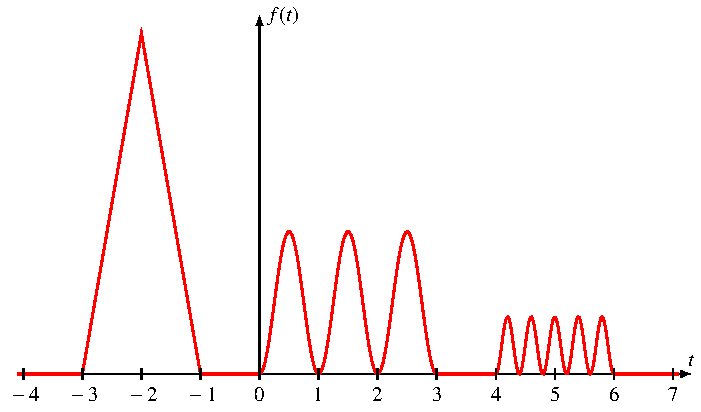
\includegraphics{chapters/4-cwt/images/f.pdf}
\caption{Funktion $f(t)$ aus \cite[p.~60]{buch:blatter}
\label{cwt:blatterfgraph}}
\end{figure}
\begin{figure}
\centering
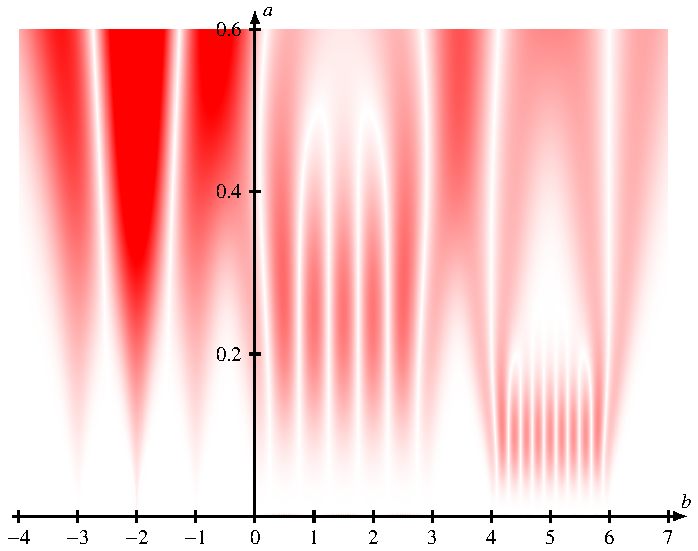
\includegraphics{chapters/4-cwt/images/notes.pdf}
\caption{Stetige Wavelet-Transformation der Funktion \eqref{cwt:blatterf}
(Graph in Abbildung~\ref{cwt:blatterfgraph}).
\label{cwt:blattercwt}}
\end{figure}
Wir berechnen die Wavelet-Transformation der folgenden Funktion $f$
für das Mexikanerhut-Wavelet \eqref{wavelet:mexikanerhut}, wir setzen also
$\psi=\psi_\text{M}$.
\begin{equation}
f(t) = \begin{cases}
2.883 \cdot (2 - 2\,|t+2|)&\qquad -3\le t \le -1\\
1.205\cdot (1-\cos(2\pi t))&\qquad 0\le t \le 3\\
0.968\cdot \frac12(1-\cos(5\pi t))&\qquad 4\le t \le 6\\
0&\qquad\text{sonst.}
\end{cases}
\label{cwt:blatterf}
\end{equation}
Eine graphische Darstellung der Funktion ist in
Abbildung~\ref{cwt:blatterfgraph} gegeben,
die numerisch berechnete Transformation ist in Abbildung~\ref{cwt:blattercwt}
dargestellt.
Die Funktion besteht aus drei Teilfunktionen, die von Intervallen getrennt sind,
in denen die Funktion verschwindet.
In den Intervallen $[0,3]$ und $[4,6]$ hat die Funktion oszillatorischen
Charakter.
Die Wavelet-Transformation ist in der Lage, dieses Verhalten zu detektieren.
Es lässt sich sogar eine ungefähre Aussage über die Frequenzverhältnisse
machen.
Die Oszillation im Intervall $[4,6]$ hat $2.5$-mal höhere Frequenz als im
Intervall $[0,3]$, was sich darin äussert, dass die Schwerpunkte der farbigen
Zonen bei etwa $2.5$-mal geringerem $a$ liegen.
\end{beispiel}

In den Abbildungen \ref{cwt:psi-cwt} und \ref{cwt:blattercwt} werden 
die Skalenfaktoren $a$ auf der vertikalen Achse abgetragen.
Grössere Werte von $a$ bedeutet dabei grössere ``Wellenlänge'' des Wavelets,
so dass die ``hochfrequenten'' Koeffizienten am unteren Rand des
Intensitätsgraphen sind.
In Anwendungen der Signalverarbeitung wird daher oft $1/a$ oder $-\log a$ 
auf der vertikalen Achse aufgetragen, so dass hohe Frequenzen wie in
einem Sonogramm weiter oben dargestellt werden.

\begin{beispiel}
In diesem Beispiel verwenden wir komplexe Morlet-Wavelets%
\footnote{Die hier gegebene Form \eqref{cwt:morlet} des Morlet Wavelets
erfüllt die Zulässigkeitsbedingung nicht, was für die folgenden 
Betrachtungen jedoch nicht von Bedeutung ist.
Mehr zum Morlet-Wavelet in Kapitel~\ref{chapter:complex}.}
\begin{equation}
\psi(t) = e^{-\frac{t^2}2 +5it}
\label{cwt:morlet}
\end{equation}
um das Sweep-Signal mit linear ansteigender Frequenz
\begin{equation}
f(t)
=
\sin(t(4+0.2t))
\label{cwt:sweep-function}
\end{equation}
zwischen $t=0$ und $t=26$.
\begin{figure}
\centering
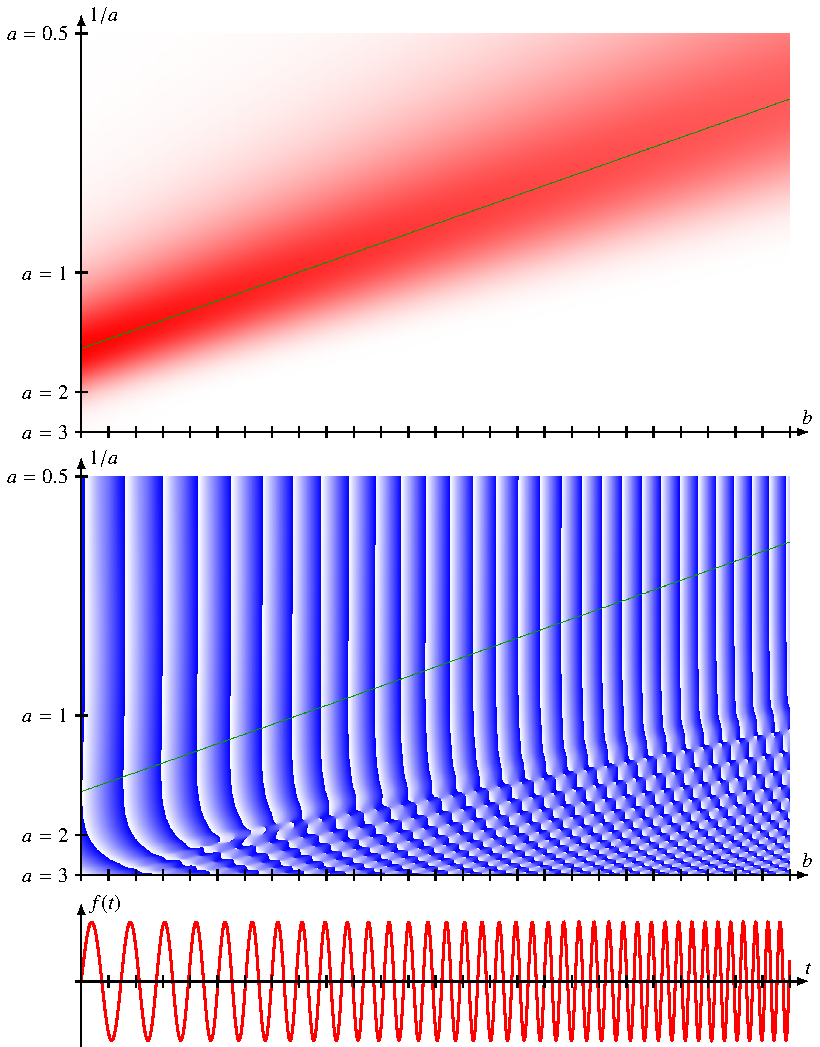
\includegraphics[width=\hsize]{chapters/4-cwt/images/sweep2.pdf}
\caption{Absolutwert und Phase der stetigen Wavelet-Transformation
der Sweep-Funktion~\eqref{cwt:sweep-function} 
für komplexe Morlet-Wavelets $\psi(t) = e^{-t^2/2+5it}$.
\label{cwt:sweep-cwt-abs-phase}}
\end{figure}
\begin{figure}
\centering
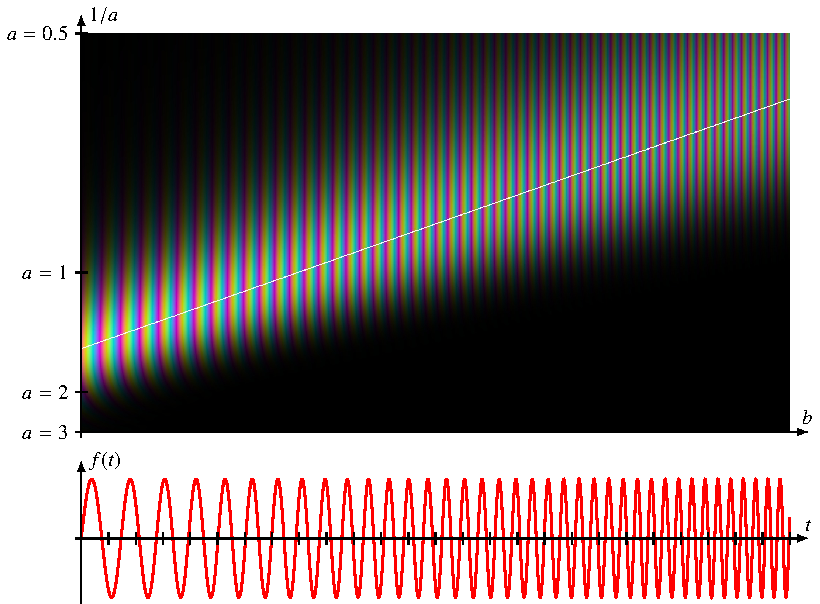
\includegraphics[width=\hsize]{chapters/4-cwt/images/sweep.pdf}
\caption{Farbcodierte Darstellung der stetigen Wavelet-Transformation
der Sweep-Funktion~\eqref{cwt:sweep-function}
für komplexe Morlet-Wavelets $\psi(t) = e^{-t^2/2} \sin(5t)$.
\label{cwt:sweep-cwt-color}}
\end{figure}
Die Resultate sind in Abbildungen~\ref{cwt:sweep-cwt-abs-phase} und
\ref{cwt:sweep-cwt-color} dargestellt.
Der Absolutwert der stetigen Wavelettransformation zeigt die aktuelle
Frequenz des Sweep-Signals an.
Das Maximum der Amplitude für jeden $b$-Wert ist in
Abbildung~\ref{cwt:sweep-cwt-abs-phase} dunkelgrün hervorgehoben.
Dank der komplexen Oszillation $e^{5it}$ ändert zwar die Phase relativ
rasch entlang des Maximums, der Absolutwert ändert dagegen nur 
langsam.
In Abbildung~\ref{cwt:sweep-cwt-color} ist die Phase durch die Farbe
codiert, auch hier wird offensichtlich, dass die Phase sehr schnell ändert,
während die Amplitude nur langsam abfällt.

Ein reelles Wavelet ergibt dagegen immer dann einen maximalen Wert der
Wavelet-Trans\-for\-ma\-tion, wenn die Extrema des Wavelets mit den Extrema
des Signals zusammenfallen.
Die komplexen Oszillation $e^{5it}=\cos 5t + i\sin 5t$ kann durch einen
Phasenfaktor immer so modifiziert werden, dass die Extrema des Realteils
mit den Extrema des Signals zusammenfallen.
Dieser Phasenfaktor hat genau die entgegengesetzte Phase der
Wavelettransformation.
\end{beispiel}
